%-------------------------
% One-page industry resume template
% Example candidate: Albert Einstein
% License: MIT
%------------------------

\documentclass[letterpaper,10pt]{article}

\usepackage[empty]{fullpage}
\usepackage[dvipsnames]{xcolor}
\definecolor{linkcolor}{RGB}{10, 80, 140}
\usepackage{titlesec}
\usepackage{enumitem}
\usepackage[normalem]{ulem}
\usepackage[colorlinks=true, urlcolor=linkcolor, linkcolor=linkcolor]{hyperref}
\usepackage{fancyhdr}
\usepackage[english]{babel}
\usepackage{tabularx}
\usepackage{fontawesome5}
\usepackage{graphicx}
\usepackage[T1]{fontenc}
\usepackage{anyfontsize}

\pagestyle{fancy}
\fancyhf{}
\renewcommand{\headrulewidth}{0pt}
\renewcommand{\footrulewidth}{0pt}

\addtolength{\oddsidemargin}{-0.60in}
\addtolength{\evensidemargin}{-0.60in}
\addtolength{\textwidth}{1.20in}
\addtolength{\topmargin}{-0.74in}
\addtolength{\textheight}{1.48in}
\setlength{\footskip}{12pt}

\urlstyle{same}
\raggedbottom
\raggedright
\setlength{\tabcolsep}{0in}
\pdfgentounicode=1

\titleformat{\section}{
  \vspace{-6pt}\scshape\raggedright\large
}{}{0em}{}[\color{linkcolor}\titlerule \vspace{-6pt}]

\newcommand{\linkicon}{{\,{\color{linkcolor}\scriptsize\faExternalLink*}}}
\newcommand{\pubicon}{{\,{\color{linkcolor}\scriptsize\faBook}}}
\newcommand{\linkedtext}[2]{\href{#1}{#2\linkicon}}
\newcommand{\paperlink}[1]{\,\href{#1}{\pubicon}}
\newcommand{\resumeItem}[1]{\item\small{#1 \vspace{-2pt}}}

\newcommand{\resumeExpHeading}[2]{
  \vspace{1pt}
  \item
    \begin{tabular*}{\textwidth}[t]{l@{\extracolsep{\fill}}r}
      \textbf{#1} & \textbf{\small #2} \\
    \end{tabular*}\vspace{-6pt}
}

\newcommand{\resumeHeading}[4]{
  \vspace{1pt}
  \item
    \begin{tabular*}{0.98\textwidth}[t]{l@{\extracolsep{\fill}}r}
      \textbf{#1} & \small #4 \\
      \textit{\small #3} & \textit{\small #2} \\
    \end{tabular*}\vspace{-7pt}
}

\newcommand{\resumeHeadingListStart}{\begin{itemize}[leftmargin=0pt, itemsep=0pt, label={}]}
\newcommand{\resumeHeadingListEnd}{\end{itemize}}
\newcommand{\resumeItemListStart}{\begin{itemize}[leftmargin=*, itemsep=1pt, topsep=1pt, parsep=0pt]}
\newcommand{\resumeItemListEnd}{\end{itemize}\vspace{-4pt}}
\newcommand{\resumeSkillSummary}[1]{{\small \textit{\uline{Skills:} #1}}\vspace{2pt}}

\begin{document}

\noindent
\begin{minipage}[t]{0.72\textwidth}
    \vspace{0pt}%
    \textbf{\Huge Albert Einstein} \\[5pt]
    \small
    Princeton, NJ \hspace{6pt} | \hspace{6pt}
    albert.einstein@example.com \hspace{6pt} | \hspace{6pt}
    +1 (609) 555-1905 \\[2pt]
    \linkedtext{https://en.wikipedia.org/wiki/Albert_Einstein}{Website} \hspace{6pt} | \hspace{6pt}
    \linkedtext{https://github.com/example}{GitHub} \hspace{6pt} | \hspace{6pt}
    \linkedtext{https://www.linkedin.com/in/example}{LinkedIn}
\end{minipage}%
\hfill
\begin{minipage}[t]{0.25\textwidth}
    \vspace{-14pt}%
    \raggedleft
    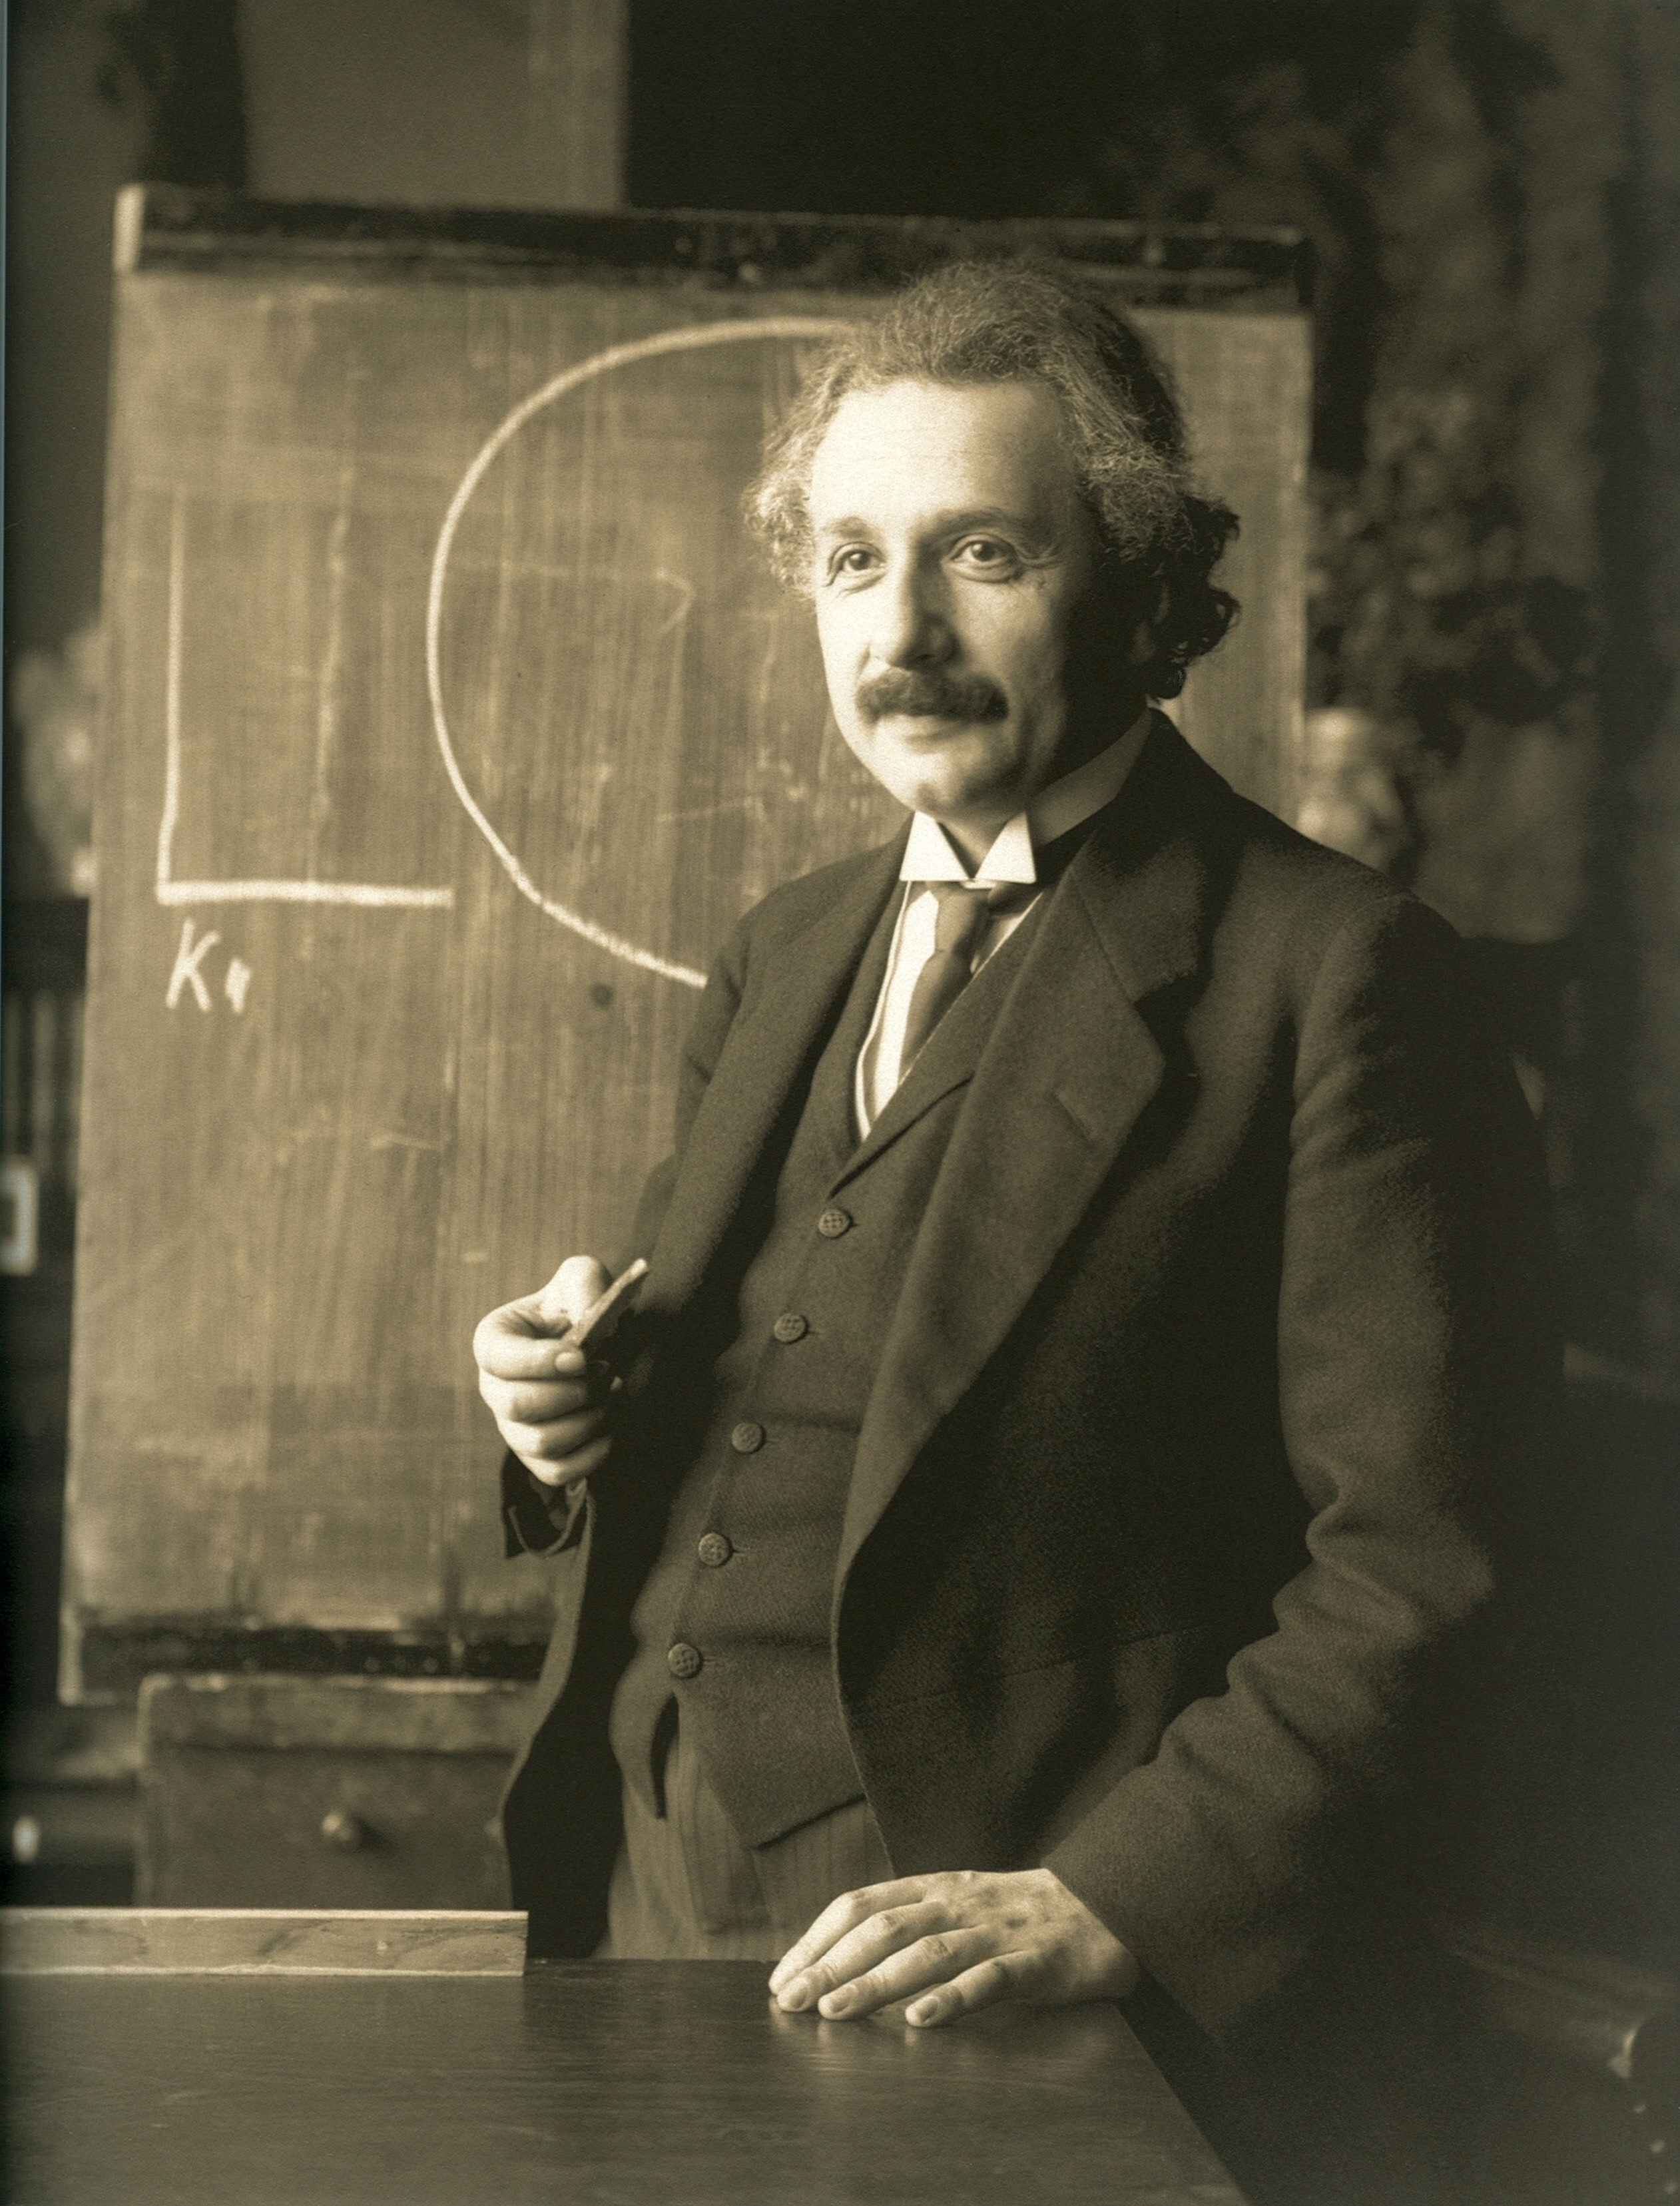
\includegraphics[width=2.6cm,height=2.6cm,keepaspectratio]{assets/einstein.jpg}
\end{minipage}
\vspace{-4pt}

\section{Experience}
\resumeHeadingListStart

  \resumeExpHeading{Senior Theoretical Researcher --- Institute for Advanced Study, Princeton}{1933 -- 1955}
  \resumeItemListStart
      \resumeItem{Built mathematical models of gravitation and field theory, translating ambiguous physical observations into testable quantitative frameworks.}
      \resumeItem{Led independent research programs across relativity, quantum theory, and statistical physics while collaborating with international scientific teams.}
      \resumeItem{Communicated complex technical ideas through papers, lectures, and public-facing writing for expert and non-expert audiences.}
  \resumeItemListEnd
  \resumeSkillSummary{Mathematical Modeling, Research Strategy, Scientific Communication, Cross-Functional Collaboration}

  \resumeExpHeading{Professor / Academy Member --- Prussian Academy of Sciences, Berlin}{1914 -- 1933}
  \resumeItemListStart
      \resumeItem{Developed the general theory of relativity, creating a predictive model that explained gravitational lensing, orbital precession, and cosmological dynamics.}
      \resumeItem{Designed thought experiments and analytical workflows to challenge assumptions, reduce hidden variables, and surface falsifiable predictions.}
      \resumeItem{Mentored researchers and coordinated seminar discussions across theoretical physics, astronomy, and applied mathematics.}
  \resumeItemListEnd
  \resumeSkillSummary{Theory Design, Problem Decomposition, Mentorship, Systems Thinking}

  \resumeExpHeading{Technical Expert --- Swiss Patent Office, Bern}{1902 -- 1909}
  \resumeItemListStart
      \resumeItem{Reviewed electromechanical patents for novelty, implementation feasibility, and technical clarity under strict documentation standards.}
      \resumeItem{Evaluated synchronization, signal transmission, and measurement systems, improving ability to reason from engineering constraints to core principles.}
      \resumeItem{Produced concise technical decisions for high-volume applications while maintaining accuracy and repeatable review criteria.}
  \resumeItemListEnd
  \resumeSkillSummary{Technical Review, Electromechanical Systems, Documentation, Prior-Art Analysis}

\resumeHeadingListEnd

\section{Selected Projects}
\resumeItemListStart
    \resumeItem{\textbf{General Relativity} -- Unified acceleration and gravity into a geometric theory with measurable astronomical predictions.}
    \resumeItem{\textbf{Photoelectric Effect} -- Modeled light quanta to explain electron emission behavior and support modern quantum theory.}
    \resumeItem{\textbf{Brownian Motion} -- Converted microscopic particle motion into statistical evidence for atomic theory.}
    \resumeItem{\textbf{Mass-Energy Equivalence} -- Derived a compact relationship connecting mass and energy across physical systems.}
\resumeItemListEnd

\section{Technical Skills}
\begin{itemize}[leftmargin=0.2em, labelsep=0pt, label={}, itemsep=0pt, parsep=0pt, topsep=1pt]
    \item \small \textbf{Core:} Mathematical modeling, analytical reasoning, uncertainty reduction, hypothesis testing
    \item \small \textbf{Domains:} Relativity, quantum theory, statistical mechanics, electrodynamics, cosmology
    \item \small \textbf{Methods:} Differential geometry, tensor calculus, stochastic processes, dimensional analysis
    \item \small \textbf{Tools:} Technical writing, patent review, lecture design, peer review, public communication
    \item \small \textbf{Languages:} German, English, French, Italian
\end{itemize}

\section{Awards \& Honors}
\resumeItemListStart
    \resumeItem{\textbf{Nobel Prize in Physics} -- Awarded for services to theoretical physics and discovery of the law of the photoelectric effect (1921)}
    \resumeItem{\textbf{Copley Medal} -- Royal Society recognition for outstanding scientific achievement (1925)}
\resumeItemListEnd

\section{Education}
\resumeHeadingListStart
  \resumeHeading
    {University of Zurich}
    {Zurich, Switzerland}
    {Ph.D. in Physics}
    {1905}
  \resumeHeading
    {Swiss Federal Polytechnic}
    {Zurich, Switzerland}
    {Diploma in Mathematics and Physics}
    {1896 -- 1900}
\resumeHeadingListEnd

\section{Selected Publications}
\begin{enumerate}[leftmargin=1.5em, label=\arabic*., itemsep=1pt, topsep=1pt]
    \item \small Einstein, A. (1916). The Foundation of the General Theory of Relativity.\paperlink{https://doi.org/10.1002/andp.19163540702}
    \item \small Einstein, A. (1905). On a Heuristic Point of View Concerning the Production and Transformation of Light.\paperlink{https://doi.org/10.1002/andp.19053220607}
    \item \small Einstein, A. (1905). On the Electrodynamics of Moving Bodies.\paperlink{https://inspirehep.net/literature/4181}
\end{enumerate}

\end{document}
